\section{验证方案与实验结果}

\subsection{验证矩阵}

项目围绕“功能正确、性能可信、实现可落地”建立了分层验证矩阵：
\begin{itemize}
    \item Smoke 回归：快速确认主线脚本、编译链路和最小软件路径可运行；
    \item Baseline \texttt{riscv-tests}：验证当前主线 ISA 集合的基本正确性；
    \item 扩展 \texttt{full-ui}：展示工程在更广测试覆盖下的稳定性；
    \item CoreMark short 与 strict：评估性能结果并验证长时间运行稳定性；
    \item Vivado \texttt{impl50} 与 FPGA-like probe：评估 FPGA 原型可实现性和路径一致性。
\end{itemize}

\begin{figure}[H]
    \centering
    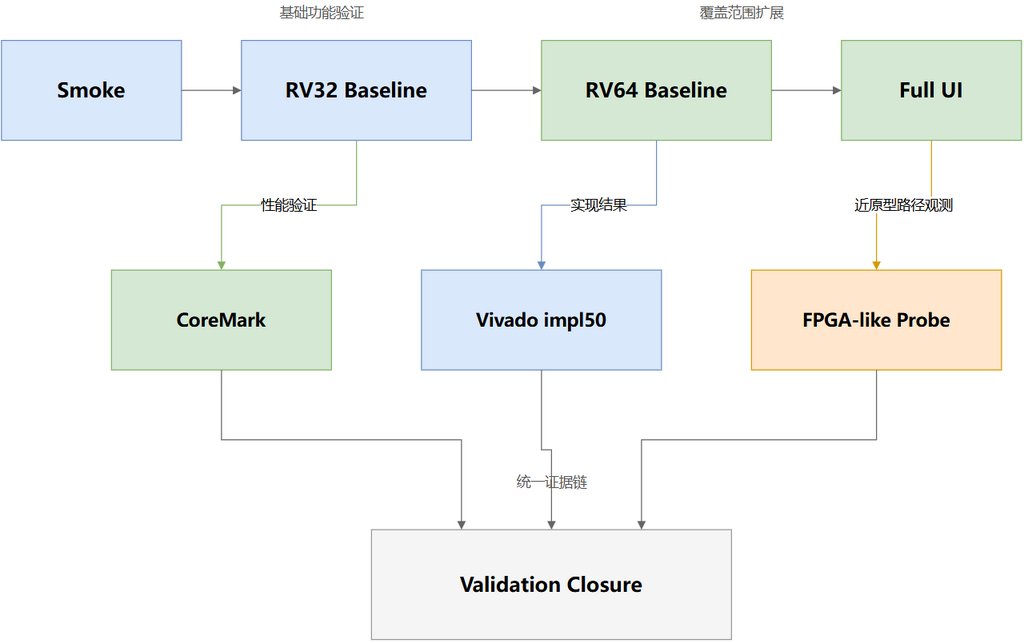
\includegraphics[width=0.96\textwidth]{figures/03-validation-closure-ai.png}
    \caption{验证矩阵与证据闭环示意图}
\end{figure}


\subsection{功能验证结果}

当前主线 baseline 回归结果如下：
\begin{table}[H]
    \centering
    \small
    \caption{主线 baseline 回归结果}
    \begin{tabularx}{0.92\textwidth}{L{0.32\textwidth} L{0.18\textwidth} Y}
        \toprule
        验证项 & 结果 & 说明 \\
        \midrule
        \texttt{rv32 baseline} & \texttt{33/33} & 当前主线 RV32 基本集合全部通过 \\
        \texttt{rv64 baseline} & \texttt{21/21} & 当前主线 RV64 基本集合全部通过 \\
        Smoke 回归 & PASS & 关键脚本与最小 SoC 软件路径运行正常 \\
        \bottomrule
    \end{tabularx}
\end{table}

为了进一步说明工程的健壮性，项目还完成了扩展 \texttt{full-ui} 覆盖：
\begin{table}[H]
    \centering
    \small
    \caption{扩展 \texttt{full-ui} 验证结果}
    \begin{tabularx}{0.92\textwidth}{L{0.26\textwidth} L{0.18\textwidth} Y}
        \toprule
        验证项 & 结果 & 说明 \\
        \midrule
        \texttt{rv32 full-ui} & \texttt{42/42} & 覆盖更广的 RV32 用户态测试集合 \\
        \texttt{rv64 full-ui} & \texttt{54/54} & 覆盖更广的 RV64 用户态测试集合 \\
        \texttt{fence\_i} 相关用例 & PASS & 作为扩展覆盖记录，用于说明测试环境适配能力 \\
        \bottomrule
    \end{tabularx}
\end{table}

\subsection{CoreMark 性能结果}

CoreMark 采用“short + strict”两条路径记录性能：
\begin{table}[H]
    \centering
    \small
    \caption{CoreMark 结果汇总}
    \begin{tabularx}{0.95\textwidth}{L{0.25\textwidth} L{0.22\textwidth} L{0.22\textwidth} Y}
        \toprule
        路径 & Score & 周期数 & 说明 \\
        \midrule
        CoreMark short & \texttt{0.912472 CoreMark/MHz} & \texttt{11014885} & 当前短跑主线结果 \\
        CoreMark strict \texttt{>=10s} & \texttt{0.912465 CoreMark/MHz} & \texttt{1095991523} & 满足 EEMBC 10s 口径 \\
        FPGA-like probe & \texttt{7.728811 CoreMark/MHz} & \texttt{156442} & 用于观察 FPGA 路径下的相对效率 \\
        \bottomrule
    \end{tabularx}
\end{table}

可以看到，short 与 strict 两条路径的 Score 保持一致性，说明当前主线在长时间运行下没有出现明显性能漂移，
也支撑了本文对结果稳定性的说明。

\subsection{FPGA 实现结果}

为了支撑 FPGA 原型评估，项目完成了 Vivado \texttt{impl50} 结果收集：
\begin{table}[H]
    \centering
    \small
    \caption{Vivado \texttt{impl50} 结果}
    \begin{tabularx}{0.92\textwidth}{L{0.32\textwidth} L{0.18\textwidth} Y}
        \toprule
        指标 & 结果 & 说明 \\
        \midrule
        Slice LUTs & \texttt{2556} & 主线资源占用 \\
        Slice Registers & \texttt{2170} & 主线寄存器占用 \\
        Block RAM Tile & \texttt{4} & 主线片上存储资源 \\
        DSP & \texttt{0} & 未依赖 DSP 资源 \\
        WNS & \texttt{+5.822ns} & 50MHz 目标下保持正裕量 \\
        WHS & \texttt{+0.057ns} & 保持正保持时间裕量 \\
        \bottomrule
    \end{tabularx}
\end{table}

\subsection{验证结论}

从当前验证矩阵可以得出三点结论：
\begin{enumerate}
    \item 主线方案在基本 ISA 正确性、CoreMark 性能和 FPGA 实现结果之间已经形成一致的证据链；
    \item 扩展覆盖结果说明该工程不仅能完成主线要求，也具备进一步拓展测试范围的稳定基础；
    \item 当前结果可以支撑初赛阶段的正式设计说明，但实体板卡相关结论仍保留在后续工作范围内。
\end{enumerate}
